\documentclass{article}
\usepackage[MeX]{polski}
\usepackage{parskip}
\usepackage{graphicx}
\usepackage[utf8]{inputenc}


\DeclareGraphicsExtensions{.pdf,.png,.jpg}


\title{Portal blogowy}
\author{\textsc{Paweł Sołtysiak I1-41A} \\ \texttt{psoltysiak@wi.zut.edu.pl}}
\begin{document}
\maketitle
\section{Wstęp}
Portal blogowy ma być platformą łącząca twórców blogów. Wspomagających ich komunikację oraz stanowić sposób na wypromowanie własnej twórczości wobec innych użytkowników portalu.



\section{Wymagania funkcjonalny}
\subsection{Tworzenie kont użytkowników}
Portal musi posiadać możliwość zakładanie kont użytkowników. Użytkowników dzieli się następujące grupy.
\begin{itemize}
\item Normalni -- osoby posiadają możliwość tworzenia blogów, usuwania własnych blogów, posiadają prawo do wprowadzania modyfikacji w własnych blogach. Posiadają możliwość wstawiania komentarzy w blogu.
\item Administratorzy -- mają pełne prawa w portalu, mogą tworzyć własne blogi mogę usuwać blogi innych osób, nie mogą edytować zawartości innych blogów.
\end{itemize}

Dane potrzebne do stworzenia konta użytkownika przypisanego do grupy normalnej:
\begin{itemize}
\item Login
\item Hasło
\item Hasło ponownie
\item Adres Email
\end{itemize}

Po wpisaniu danych do formularza tworzącego konto, musi zachodzić sprawdzenie poprawności danych wpisanych przez użytkownika. W tym przypadku Login nie może się powtarzać, hasło i hasło wpisane ponownie musi być jednakowe oraz wpisany adres Email musi być poprawnym adresem email.

Przy powstaniu serwisu blogowego musi istnieć przynajmniej 1 konto użytkownika z uprawnieniami administratora. Następne konta z grupy Normalnej będą mogły dostać zwiększone uprawnienia przez jednego z administratorów.

\subsection{Tworzenie blogów}
Portalu musi posiadać funkcjonalność zakładania własnych blogów. Każdy blog jest przypisany do jednej konkretnej osoby. Właściciel bloga może z własnego bloga dodawać nowe treści do bloga, zwanymi także Wpisami, poprzez edytor typu WYSIWYG (ang. What You See Is What You Get). Oprócz treści wpisu użytkownik musi podać tytuł oraz określić kategorię wpisu.

Każdy z stworzonych wpisów powinien pozwalać na edycję zapisanego wpisu.

Użytkownik powinien posiadać możliwość na usuwanie wcześniej stworzonych Wpisów. Do tego powinien służyć przycisk w ostrzegającym kolorze, po którym powinno się wyświetlać okno potwierdzające decyzję użytkownika.

\subsection{Komentarze}
Każdy z użytkowników przypisanych do grupy Normalnej posiada możliwość zostawiana komentarzy pod wpisami blogowymi.

Każdy wpis na każdym blogu powinien podlegać możliwości komentowania.

Twórca komentarzu powinien mieć możliwość usunięcia wprowadzonego komentarza.

\section{Wymagania niefunkcjonalne}
System pownien być dostępny poprzez przeglądarkę internetową 

System powinien działać niezależnie od systemu operacyjnego użytkownika.

System powinien zostać stworzony oparciu o technologię .NET oraz z wykorzystaniem bazy danych SQL Server.


\section{Diagram przypadków użycia}
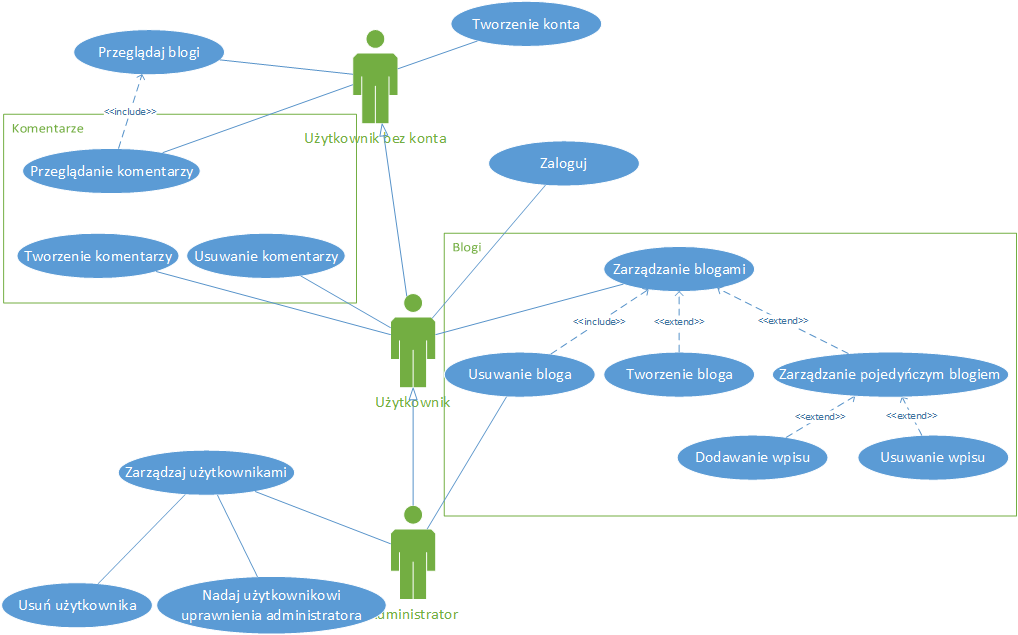
\includegraphics[width=\textwidth]{UseCaseDiagram}
%next-next exam
\section{Diagram klas}
\subsection{Diagram repozytoriów}
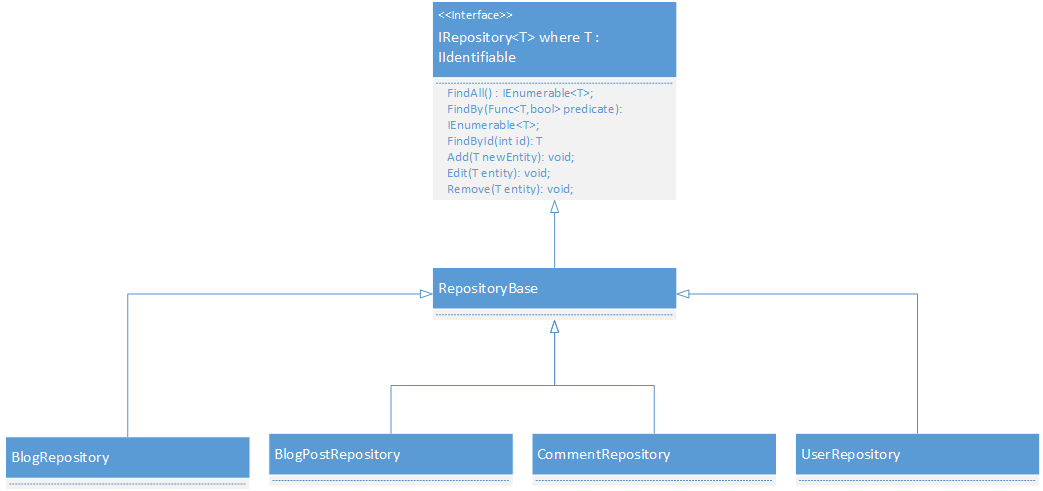
\includegraphics[width=\textwidth]{RepositoryClassDiagram}
\subsection{Diagram modelu}
\section{Diagram komponentów}

\end{document}

